\chapter{Developer Documentation}

In this chapter we aim to describe the implementation of the demo version of our game.
In the first section~\ref{sec:docs-proj} we describe the overall structure, and in the later sections we go into more detail about the individual parts.
Section~\ref{sec:docs-battle} describes what goes on from the application start to the end, including all procedural generation, but not what happens during a battle.
We will focus on battles first, in section~\ref{sec:docs-data}.

\section{Project Structure}\label{sec:docs-proj}

In Unity, each project is composed of individual scenes.
The scenes contain game objects to which are attached scripts that provide their behavior.
These are all saved in the project's asset folder, along with all other resources like prefabs, models, materials, textures, sounds and more.
They are separated to folders based on their type, for example all scenes are in the \emph{Scenes} folder.

In addition to the project assets, an important part of the project are the project settings.
However, these are all mostly set to their default value from the standard \emph{3D (Built-in render pipeline)} project template.
The settings that were changed are all uninteresting adjustments that an experienced Unity user would expect us to configure how we did, based on the explanation of our project provided in this chapter and chapter~\ref{analysis}.
These include for example settings in categories \emph{Tags and Layers}, \emph{Physics} and \emph{Player}.

\subsection{Scenes}

The demo version of our game is composed of 5 scenes.
We provide a brief summary of each, but we will describe them in more detail later.
This summary will be useful for the rest of the chapter, allowing us to see which parts of the game occur chronologically after other parts.
For convenience, the transitions between the scenes are shown in figure~\ref{fig:scene-transitions}.
\begin{itemize}
    \item \textbf{Loading} is the first scene that gets loaded when the game starts.
          This scene contains only scripts that load data and game objects that persist throughout the entire lifetime of the application.
          After the loading is done, this scene transitions to \emph{Menu}.
    \item \textbf{Menu} contains the game title, and a button to start a run, a button to set up a custom run, and a button to exit the game.
          The start button takes the player to the \emph{Battle} scene, whereas the custom run button leads to the \emph{Run Settings} scene.
    \item \textbf{Run Settings} lets the player customize the run by selecting a custom seed or by opting to select their starting blueprints.
          There is also a button that lets the player play again the in-game tutorial.
          Starting a run from here also takes the player to the \emph{Battle} scene, unless they chose to select starting blueprints in which case they go to the \emph{Blueprint Selection} scene.
    \item \textbf{Battle} is the scene where the battles happen.
          Here the player plays one level of the game as described in previous sections, until they win the level or lose.
          If they lose, their only option is to return to \emph{Menu}.
          When they win, they continue to the \emph{Blueprint Selection} scene.
    \item In \textbf{Blueprint Selection}, the player is shown their current blueprints and new blueprints to choose from.
          When they finish choosing, they continue to the next \emph{Battle}.
\end{itemize}


\begin{center}
    \captionsetup{type=figure}
    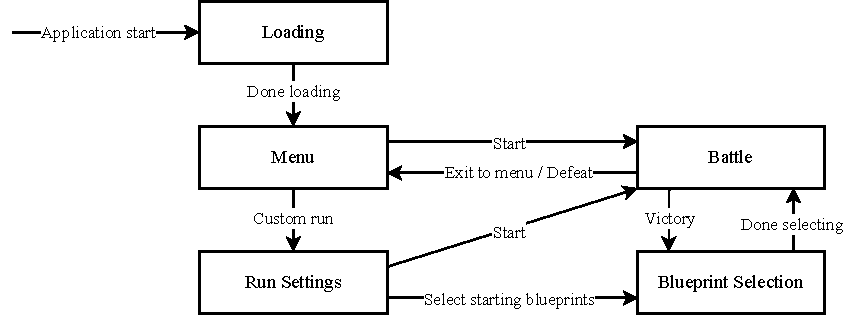
\includegraphics[width=0.9\textwidth]{img/Scene transitions.pdf}
    \caption{Scene transitions.}
    \label{fig:scene-transitions}
\end{center}


\subsection{Scripts}

There are some game objects which persist between scene transitions, but most of them are confined only to one scene.
Each battle happens in one scene, but it still contains multiple systems which are loosely coupled.
The structure of the project and its systems is reflected in the structure of the \emph{Scripts} folder.
The scripts are also separated into namespaces and assemblies based on this structure.
In the later sections of this chapter we describe how the scripts interact.

We would also like to mention that in the code, in \mono{MonoBehaviour} scripts, we use some conventions that might seem odd to programmers who don't use Unity.
For example, many private fields have the attribute \mono{[SerializeField]} which makes them show up in the Unity editor in the inspector.
This lets us save the values of these fields as a part of the scene, instead of initializing them in code.
We can also inspect the value of these fields at runtime in the Unity editor.
Since properties don't show up in the inspector, we use public fields in many places where it would be more appropriate to use a property with a public getter and a private setter.

\iffalse
    \begin{figure}[H]
        \centering
        \begin{forest}
            forked edges,
            for tree={
                    grow'=east,
                    anchor=base west,
                    l sep+=0.5em,
                    fork sep=0.5em,
                    tier/.option=level,
                    calign=first,
                    s sep=0mm
                },
            parent anchor=east,
            [Scripts
                        [\mono{BattleSimulation}
                            [\mono{Abilities}]
                            [\mono{Attackers}]
                            [\mono{Buildings}]
                            [\mono{Control}]
                            [\mono{Projectiles}]
                            [\mono{Selection}]
                            [\mono{Targeting}]
                            [\mono{Towers}]
                            [\mono{World}
                                [\mono{WorldBuilder}]
                                [\mono{WorldData}]
                            ]
                        ]
                        [\mono{BattleVisuals}
                            [\mono{Abilities}]
                            [\mono{Attackers}]
                            [\mono{Camera}]
                            [\mono{Effects}]
                            [\mono{Projectiles}]
                            [\mono{Selection}
                                [\mono{Highlightable}]
                            ]
                            [\mono{Towers}]
                            [\mono{UI}]
                            [\mono{World}]
                        ]
                        [\mono{Data}
                            [\mono{Loader}]
                            [\mono{Parsers}]
                            [\mono{WorldGen}]
                        ]
                        [\mono{Game}
                            [\mono{AttackerStats}]
                            [\mono{Blueprint}]
                            [\mono{InfoPanel}]
                            [\mono{Run}
                                [\mono{Events}]
                            ]
                            [\mono{Shared}]
                            [\mono{Tutorial}]
                        ]
                        [\mono{Utils}
                            [\mono{DotNetHacks}]
                            [\mono{Random}]
                        ]
                        [\mono{WorldGen}
                            [\mono{Decorations}]
                            [\mono{Obstacles}]
                            [\mono{Path}]
                            [\mono{WFC}]
                            [\mono{WorldSettings}]
                        ]
                ]
        \end{forest}
        \caption{Namespace and folder structure of our scripts.}
        \label{fig:proj}
    \end{figure}

    We also name the namespaces in our project according to the folder structure.
    Furthermore, the project is split into assemblies, where each folder is basically one assembly.
    However, assembly references can't form cycles, so all scripts in the folder \mono{WorldGen}, except for the subfolder \mono{WorldSettings} are one assembly.
    Furthermore, there are a few assemblies that contain only one interface, which facilitates dependency inversion in places where we would need to create a cycle in assembly references.
    These are \mono{BattleVisuals.Selection.Highlightable} and \mono{Data.Loader}.

    Here, we provide a short overview of the top level script folders and the implementation of the systems they contain:
    \begin{itemize}
        \item \nameref{sec:docs-sim}~--- game logic of all systems that are contained in a battle.
        \item \nameref{sec:docs-vis}~--- logic for the visuals during a battle like animations, particle effects and the user interface.
        \item \nameref{sec:docs-data}~--- parsing and loading data in the \emph{Loading} scene.
        \item \nameref{sec:docs-game}~--- systems and concepts that are present outside battle, across multiple battles or throughout the whole application runtime.
        \item \nameref{sec:docs-utils}~--- various utility functions and data structures used throughout the project.
        \item \nameref{sec:docs-worldgen}~--- procedural generation of the world for each level.
    \end{itemize}
    The following sections of this chapter will go into more detail.

\fi


\subsection{Third-Party Assets}
In the project, we use some assets that were not created by the author of this thesis in addition to the Unity game engine.
We would like to acknowledge and disclaim these assets here:
\begin{itemize}
    \item The Unity package \textbf{UI Soft Mask} by \emph{mob-sakai}~\cite{SoftMask}.
    \item We adapted the implementation of a \textbf{Priority Queue} from the \emph{.NET Platform}~\cite{PriorityQueue}.
    \item We also adapted an \textbf{Editor Init} script by \emph{Z4urce}~\cite{EditorInit}, used to select the scene to load when we run the game in the Unity editor.
    \item And a function for calculating the number of set bits in an \mono{int}, or \textbf{Hamming Weight}, from this \emph{stack overflow} answer~\cite{PopCount}.
    \item The font used for all text in the game is \textbf{Open Sans} by the \emph{Open Sans Project contributors}~\cite{OpenSans}.
\end{itemize}

\section{Battle}\label{sec:docs-battle}

During a battle, the game reacts to the player's inputs, so a battle cannot be viewed as a linear program, which takes inputs and transforms them into outputs.
Instead, there are shorter procedures happening all the time, triggered either by the player's inputs or in-game events, which modify the state of the game.
Also, many game objects autonomously repeat a simple procedure every frame, for example, an attacker moves some distance along its path every tick.
We will describe these procedures in the following subsections.
First, we will describe the game logic, and in the later sections we will explain how the game visuals work.

In this section we assume the world is already generated and the game is ready for the player's inputs.
The scene is composed of the generated world, the UI and singleton objects with scripts that handle the global game systems.
For example, the \mono{BattleController} keeps track of the player's resources and whether the player has won or lost this battle.
Or the \mono{BlueprintMenu}, which holds the blueprints available to the player and their current cooldowns.
There are also singletons which don't come from the \emph{Battle} scene, but persist between the scenes.
For example, \mono{RunPersistence} keeps track of the player's hull and their blueprint collection.

\subsection{Selecting a Blueprint}

First, we'll take a look at what happens when the player selects a blueprint.
Let's assume they select the blueprint by clicking on it in the blueprint menu.
To click on it, the player will first have to position the mouse cursor over the blueprint, and even that triggers some reactions.

Each blueprint in the blueprint menu is an instance of the \emph{BlueprintMenuItem} prefab.
They were created by the script \mono{BlueprintMenuDisplay}, and during initialization, it registered mouse event callbacks to the \mono{SelectionController}.
The \mono{SelectionController} manages what object is currently selected and/or hovered over.
It gets only notified that a blueprint at some index in the blueprint menu was clicked, so it asks the \mono{BlueprintMenu} what blueprint is in the menu at this position.
Based on that, it notifies the \mono{InfoPanel} what it should display, or that it should hide when nothing is hovered or selected.

\subsection{Placing a Blueprint}

When a given blueprint gets selected, the \mono{SelectionController} instantiates its associated prefab.
However, the blueprinted objects are programmed with this in mind, so for example, a tower won't shoot at attackers until it's actually placed.
Also, the visual parts of the buildings or abilities start disables, so they are not visible, and their scripts don't run.
If the blueprint gets deselected without placing it, the blueprinted object gets destroyed.

When \mono{SelectionController} instantiates the blueprinted object, it finds a \mono{Placement} script on it.
\mono{Placement} is an abstract class and its derived classes implement the logic for where can this blueprint be placed.
At every \mono{Update()}, the \mono{Selection} controller gives the \mono{Placement} information about what's the mouse cursor currently hovered over, and the \mono{Placement} positions the object as if it was placed right now.
Thanks to this, we can show if the placement is valid or the updated information about the object if it would be affected for example by a special building.

When the player clicks to place the selected blueprint, \mono{SelectionController} asks \mono{BlueprintMenu} if the blueprint is ready to be placed, and the \mono{Placement} if this position is valid.
If this succeeds, the \mono{BlueprintMenu} and \mono{Placement} are notified, and the \mono{SelectionController} deselects the blueprint.
Here, \mono{BlueprintMenu} communicates with \mono{BattleController} using its modifiable queries and commands (see section~\ref{sec:analysis-modifiable-commands}) to know whether the player can afford the given blueprint, and then to pay the blueprint's cost.
\mono{BlueprintMenu} also keeps track of the blueprints' cooldowns.

When the \mono{Placement} script is told to place the blueprint, it relays this to the \mono{Blueprinted} script.
\mono{Blueprinted} is an abstract class whose derived classes implement the behavior of the given blueprinted object.
Each building or ability uses a different implementation, which is processed mainly during \mono{FixedUpdate()}.

Buildings also often register modifiers or reactions to some modifiable query or command when placed.
For example, most production blueprints produce resources every turn, so they register a modifier to the modifiable query which asks for the production par turn.
They also register a reaction to the event that a wave has ended, because they produce the resources specifically after every wave.

\subsection{Wave}

Waves are handled by the \mono{WaveController} script.
When the player requests to start a new wave, it invokes the \mono{START\_WAVE} modifiable command.
This command has modifiers that check if it's valid to start a new wave, and it also has reactions, for example the \mono{BlueprintMenu} switches which blueprints are available from buildings to abilities.

When the wave is started, the \mono{WaveController} requests the contents of the wave from the \mono{WaveGenerator}, and it starts spawning the specified attackers.
To spawn an attacker, it instantiates the prefab specified by the attacker stats, and it initializes the attacker's \mono{Attacker} script.
The attackers then move and behave on their own, as implemented in their \mono{Attacker} script.

The \mono{WaveController} does not keep track of the attackers, only their count.
Whenever it spawns an attacker, it increments the count, and whenever an attacker dies or reaches the Hub, the count is decremented.
Once all attackers have been spawned, and there are no attackers left, the wave ends, and the \mono{ON\_WAVE\_FINISHED} event is invoked.
This event has many reactions, for example the \mono{BlueprintMenu} switches the blueprint offer back to buildings, and it decrements all cooldowns
Also, this is when most production buildings produce resources.

Whenever an attacker reaches the Hub, before destroying itself and reporting it to the \mono{WaveController}, it also invokes the command \mono{damageHull} in \mono{RunEvents}, so \mono{RunPersistence} can decrease the player's hull.
If the hull reaches 0, the command \mono{defeat} is invoked.
This lets all game systems know that they should stop, and to display the \emph{defeat} overlay.

Similarly, once the player's fuel amount reaches the goal, \mono{BattleController} invokes the \mono{WIN\_LEVEL} command.
This also makes most systems from working and displays the \emph{victory} overlay.
When the player clicks the \enquote{Next Level} button, the \mono{BattleController} notifies the \mono{RunPersistence} to go to the next level.

\subsection{Shooting at Attackers}

As we described in section~\ref{sec:analysis-targeting}, when an attacker collider enters a targeting collider, the \mono{TargetingCollider} script finds the \mono{Attacker} script attached to the attacker.
The \mono{Targeting} script on a tower can have many \mono{TargetingCollider}s as children, and they can be combined with any boolean operations to create various range shapes.
Only when the attacker enters the actual range of the tower, the \mono{Targetting} adds it to its list of attackers in range, and analogously, it gets removed from the list when it leaves the range.

Most towers don't care about an attacker entering or leaving their range.
Instead, they check every tick they could shoot if they have a target, and if so, they shoot at it.
Some towers hit their target instantly, but others shoot a projectile, which will take few ticks to hit the target, or it might even miss.
The behavior of various projectiles is implemented in the derived classes of \mono{Projectile} used in their prefabs.
Once they hit their target, they notify the tower they originated from.

To hit an attacker, the tower asks whether this really was a hit, using the \mono{HIT} command for the given attacker.
If it was a hit, it then tries to damage the attacker using the \mono{DAMAGE} command.
Similarly, when the player uses an ability to damage attackers, the ability determines its targets, usually using a sphere cast, and tries to \mono{HIT} and \mono{DAMAGE} them.

\subsection{Info Panel and Blueprints}

The info panel exists both in the \emph{Battle} and \emph{Blueprint Selection} scene, and the public methods of the \mono{InfoPanel} script get called directly by various scripts.
To show info about a certain object, the right method is called, and the object is passed as an argument.
The info panel is then set up accordingly, including an instance of the right \mono{DescriptionProvider} script.
Every frame, it asks the \mono{DescriptionProvider} for the current description.
Each \mono{DescriptionProvider} first generates the description with tags as specified in section~\ref{sec:analysis-description-tags}, and then it uses the \mono{DescriptionFormatter} to format them into the corresponding formatted text and icons.

Many tags used in the descriptions of buildings or blueprints represent a value that can be modified.
The \mono{Blueprint} script contains a modifiable query for each modifiable value it holds.
The values stored in the blueprint are the base values, and the real up-to-date values are to be obtained through these queries.
For formatting the descriptions, the \mono{DescriptionFormatter} compares these modified values to the base values, and it colors the text based on if the modified value has changed for the better, worse or not at all.

The info panel also shows some control buttons when a building is selected.
It shows a delete button to delete the building, and for towers, it also shows arrow buttons that allow the player to change the tower's targeting priority.
Since the info panel has a reference to the building it's displaying information about, it can just directly call the building's public methods for this functionality.
It's important to note that when a building gets destroyed, it has to unregister all modifiers and reactions it has registered.

\subsection{Highlights}

The \mono{HighlightController} looks at the \mono{SelectionController}'s selected and/or hovered objects every frame and determines which objects in the world should be highlighted.
If the selected object has a \mono{HighlightProvider}, or when a tile has a building with a \mono{HighlightProvider} on it, the \mono{HighlightController} asks it what \mono{IHighlightable} objects should be highlighted, and with which color.
It then tells these object to change their highlights accordingly.
Each derived class of a \mono{HighlightProvider} will have a different way of determining what should be highlighted.

It also closely communicates with the \mono{SelectionController} when placing a blueprint.
It highlights the selected tile, or attacker, or it shows just a point highlight which highlights the selected position in the world, based on the \mono{Placement}.
Also, this highlight is red for placements that would be invalid.

Each \mono{HighlightProvider} also implements a function that returns the color of the range visualization for any given point, as described in section~\ref{sec:analysis-range}.
The script \mono{RangeVisualization} then creates the range visualization over many frames, based on the \mono{HighlightProvider} that's currently selected according to the \mono{HighlightController}.

In addition to our specification in section~\ref{sec:analysis-range}, when placing a blueprint, the \mono{HighlightProvider} also shows in blue the valid positions to place it.
For this, it needs a reference to the given \mono{Placement} script.

\subsection{Visuals and Interpolation}

Each blueprinted object has some scripts that control its visuals.
These usually have a reference to the script that handles the game logic, and they read the script's public variables.
The game logic scripts also expose several Unity events we can use.

For example, the script that takes care of the visualization of most projectile-shooting towers is \mono{BasicProjectileTowerVisuals}.
It controls the rotation of the tower's turret to point towards the attacker the tower is targeting, but it also interpolates the rotation to be smooth.
It also subscribes to the tower's \mono{onShoot} Unity event to play an animation when the tower shoots.

There are also various scripts that handle the appearance of the various UI elements.
These mostly behave independently by having a reference to the relevant game logic script, and they read its variables.
Blueprint menu items each have a \mono{BlueprintDisplay} script that handles most of the behavior, but the behavior is also modified by their \mono{BlueprintMenuItem} script, which gets data from the \mono{BlueprintMenuDisplay} script.

The various visuals scripts also react to the game events.
For example, the \mono{NumberEffects} script spawns a number effect above an attacker whenever the attacker gets damaged, and it creates number effects whenever resources get produced.
These number effects show the amount of damage that was dealt, or the amount and type of the resource produced.

\subsection{Tutorial}

The tutorial is handled by a system separate from other scripts, however it calls their public methods, and modifies their data to achieve the behavior we want.
There are two scripts that handle the tutorial:

\mono{TutorialController} manages at which step of the tutorial is the player currently, and for each step, it has a Unity event that gets invoked at the start of the step.
So, all things that happen during the tutorial can be assigned in the Unity editor.

The script \mono{TutorialActions} then contains methods which do various modifications to various objects within the scene, so these actions can be subscribed to the \mono{TutorialController} Unity events.
\mono{TutorialActions} also contains various checks based on which it tells the \mono{TutorialController} when to go to the next step.

\section{Data Flow and Procedural Generation}\label{sec:docs-data}

In this section we'll take a look at the processes that happen from the application start, all the way to generating worlds and waves.

\subsection{Loading}

When the application starts, a \enquote{Made with Unity} splash screen is shown, and then the \emph{Loading} scene is loaded.
This scene contains some game objects that will persist throughout the entirety of the application runtime.
These are the \mono{SceneController} and \mono{SoundController}, each with a script of the same name attached to it.
They use the singleton design pattern and static methods to allow other scripts to use their functionality without obtaining a reference to them first.

\mono{SoundController} is used to play sounds using one function call, which is convenient, because we need to create stationary audio sources all the time.
It also pools its \emph{AudioSource} prefabs to save on resources.

\mono{SceneController} is used to change scenes.
Unity lets us change scenes with a static function call on the \mono{SceneManager}, but \mono{SceneController} fades out the screen first, then it changes the scene, and it fades back in after.

The loading scene also contains an object with the \mono{StartLoader} script, which loads various data from the disk into memory, and then it calls to change the scene to \emph{Menu}.
We can register to it any number of \mono{ILoader} scripts, which do the loading and store the data in singleton classes.

Currently, the only loader we use is \mono{TerrainTypeLoader}, which loads the terrain types from the \emph{StreamingAssets/TerrainTypes} folder.
For each terrain type file, the \mono{TerrainTypeLoader} creates a new \mono{TerrainType} object using the function \mono{Parse} it has.
The parsing is done using a simple parser implemented in the folder \emph{Scripts/Data/Parsers}.
The terrain type file format will be described in section \xxx{TODO}.

\subsection{Menus and Starting a Run}

The \emph{Menu} scene contains mostly just three buttons and an object with the \mono{RunStarter} script.
All three buttons call a method on the \mono{RunStarter} when pressed.
When the \enquote{Start} button is pressed, the \mono{RunStarter} instantiates the \emph{RunPersistence} prefab, configures it, and calls the \mono{NextLevel()} method on its \mono{RunPersistence} script.

Pressing the \enquote{Custom Run} button takes the player to the \emph{Run Settings} scene.
It contains more UI elements, but another object with a \mono{RunStarter} script is present.
Here, the player can change the run settings by interacting with the UI elements, which in turn notify the \mono{RunStarter} about these changes.
When the player starts the run, the instantiated \emph{RunPersistence} prefab is then configured according to the settings.
If the \enquote{Select starting blueprints} option is enabled, instead of going to the first level, the scene \emph{Blueprint Selection} is loaded, where the player can select the starting blueprints.

\subsection{Run Persistence and Blueprint Rewards}

The \emph{RunPersistence} object persists between scenes and only destroy itself when a run ends.
It holds all scripts that need to remember some state throughout the whole run:
The \mono{RunPersistence} script keeps track of the player's hull and blueprints, the run seed, the current level, and it gives orders to the other scripts.
When it's initialized, it also initializes the \mono{BlueprintRewardController} script with a random seed, derived from the run seed.

Whenever the \mono{RunPersistence} wants to go to the \emph{Blueprint Selection} scene, it asks the \mono{BlueprintRewardController}.
For the rewards after the first tutorial level, or when selecting starting blueprints, the \mono{BlueprintRewardController} prepares predefined blueprint selection, but for normal blueprint rewards, it picks the selection randomly, based on its seed.
It then changes the scene to the \emph{Blueprint Selection} scene, and initializes the \mono{BlueprintSelectionController} script in it with the selection.
The \mono{BlueprintSelectionController} handles the blueprint selection, and then it returns what the player chose in a callback to the \mono{RunPersistence}, which updates the player's blueprint collection.
Then, the game proceeds to the next level.

\subsection{Procedural Level Generation}

Whenever the \emph{Battle} scene is loaded, the \mono{WorldGenerator} finds the \mono{RunPersistence} and asks it to set up the level settings.
For this, the \mono{RunPersistence} uses the \mono{LevelSetter} script, which finds the relevant scripts in the scene and sets them up.
It generates a new seed for the world generator and configures the number of paths and their lengths, based on the level number, storing this information in the \mono{WorldSettings} script.
It also configures the \mono{WaveGenerator}'s seed and parameters, and the fuel goal in the \mono{BattleController}.

As we described in section~\ref{sec:analysis-rng}, we use \emph{seed branching} everywhere throughout the procedural generation.
This means that whenever some system needs RNG, it gets a seed from another system, and from this seed it creates its own RNG instance to use.
Figure~\ref{fig:seed-branching} shows how the seeds get propagated across the game's systems.

\begin{center}
    \captionsetup{type=figure}
    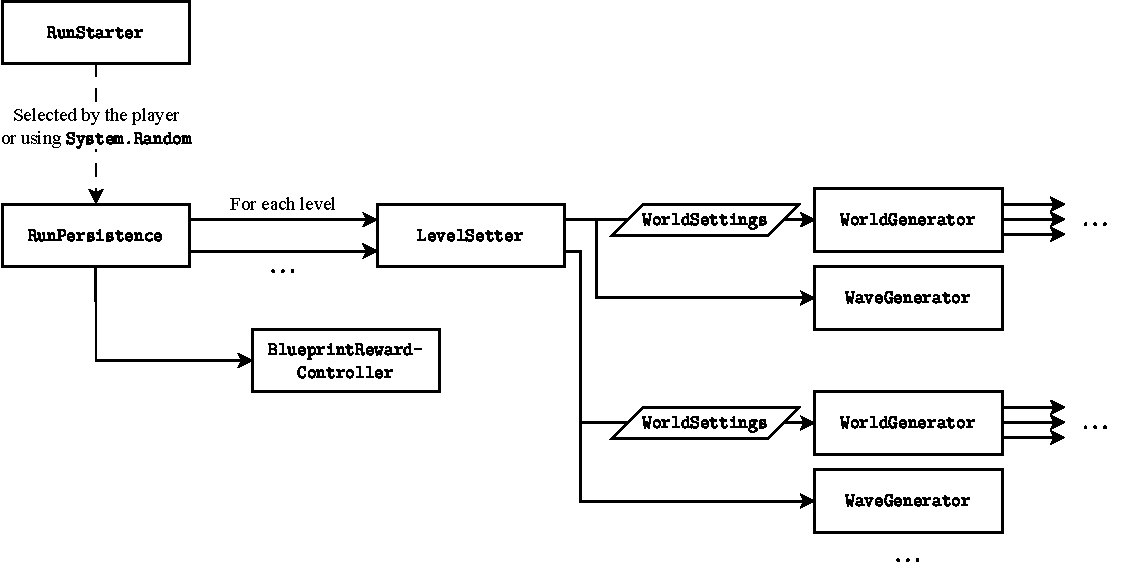
\includegraphics[width=\textwidth]{img/seed splitting.pdf}
    \caption{Seed propagation using seed branching.}
    \label{fig:seed-branching}
\end{center}

The world generator uses other scripts from the \emph{WorldGen} folder, and proceeds in steps as described in section~\ref{sec:analysis-procedural-generation}.
These steps are done in so that the game doesn't become unresponsive.
After each step, it saves the generated data int a singleton instance of \mono{WorldData}.

In Unity, we cannot instantiate objects from a background thread.
So, in the main thread, the script \mono{WorldBuilder} checks for the \mono{WorldData} being filled in, and according to those, it builds the terrain, obstacles and paths.
This is still done using Unity coroutines across multiple frames to not lag the game.
Currently, the screen is faded out using the \mono{SceneController} during world generation, but later we'd like to add an animation, which would make any stutters obvious.
